\documentclass[hidelinks]{report}

\usepackage{graphicx}
\usepackage{times}
\usepackage{plain}
\usepackage[plainpages=false]{hyperref}
\usepackage{courier}
\usepackage{caption}

% To force figures to appear after text(along with [H] option)
\usepackage{float}

% To apply linespacing to some content
\usepackage{setspace}

% To show commands, code snippets
\usepackage{listings}

% To use checkmark (tick symbol)
\usepackage{amssymb}

\graphicspath{ {images/pdf/} }

\pagestyle{plain}

\fontfamily{Times}
\selectfont

\setlength{\textwidth}{6.5in}
\setlength{\textheight}{8.5in}
\setlength{\topmargin}{-0.25in}
\setlength{\oddsidemargin}{-0.00in}
\setlength{\evensidemargin}{-0.00in}

% To use multirow feature of latex tables
\usepackage{multirow}

% Using and defining own color
\usepackage{color}
\definecolor{mycol}{RGB}{52, 43, 41}

% Defining courier font usage syntax
\newcommand{\cf}[1] {
	\textbf{\texttt{#1}}
}

% Defining checkmark usage syntax
\newcommand{\T} {
	\checkmark
}

\begin{document}
%% Line spacing 1.5 applied
\setstretch{1.5}
\section*{Developer Manual}
We have designed and implemented various IMS core modules (PCSCF, SCSCF, HSS, ICSCF) along with a RAN simulator. The whole setup can be called as an NFV-based IMS core and its block diagram is shown in figure 1. RAN
simulator is used for the purpose of generating traffic to our IMS. 

\begin{figure}[H]
\centering
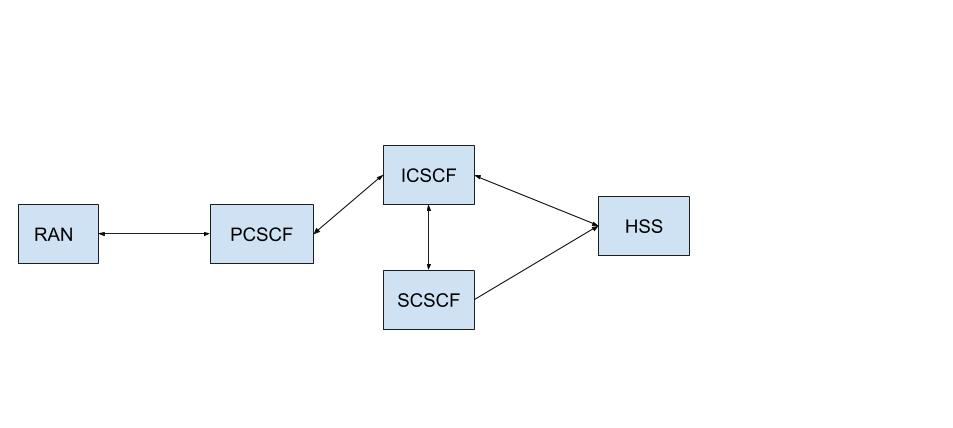
\includegraphics[scale=0.45]{IMS_Architecture.jpg}
\caption{IMS block diagram}
\label{IMSArchitecture}
\end{figure}

\section*{Overview of NFV IMS core}
All the components in IMS core (P-CSCF, I-CSCF, S-CSCF, and HSS) are epoll based and use nonblocking sockets. We made this design choice as it makes porting IMS core to mTCP easy.We made the kernel stack-based version of NFV IMS core multicore scalable by sharing listen socket between threads by adding lock before at the time of thread adds a socket to epoll for listening. We have modified packet API built by NS Sadgopan  and used it for implementing IMS core. We made following assumptions and high level  simplifications while designing IMS.
\begin{itemize}
\item Standard compliance is not our goal. So we did not implement corner cases and complexities which are not relevant for performance evaluation. For example, the standard compliant system will have multiple deregistration procedures each corresponding to multiple scenarios like HSS initiated deregistration, UE initiated deregistration. We chose UE initiated deregistration as it was enough for achieving our goal of performance evaluation. Similarly, instead of IPSec we have used the libcrypto library for encryption-decryption.
\item There is lower level connectivity process of the initial connection of UE with the access network before it can actually start the registration process. We assume that this setup is already there and UE has P-CSCF IP address where it has to connect. 
\item There are multiple identities in IMS. We have chosen to use IMSI and GRUU. These two identities are enough for our implementation. There are other identities like IMPI(IP multimedia public identity), T-GRUU(Temporary GRUU) and more which are required for scenarios which we have not implemented, so our implementation does not have it.
\subsection*{Epoll based program design}
\begin{figure}[H]
\centering
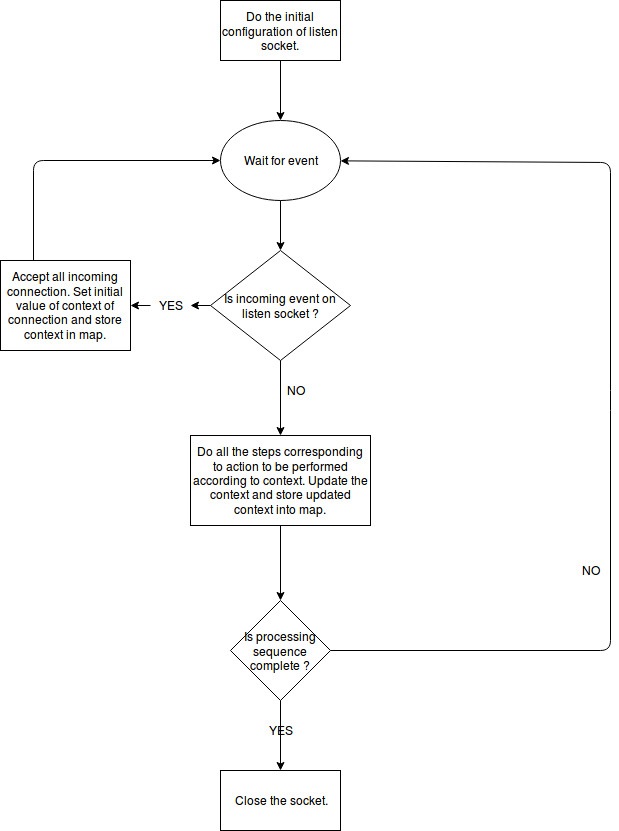
\includegraphics[scale=0.45]{Epoll_Based_Program_Flow.jpg}
\caption{Epoll based program flow}
\label{Epollbasedprogram}
\end{figure}
Figure \ref{Epollbasedprogram} shows the architecture of epoll system which we have developed.In epoll based system we need to store the state of every request which is currently executing.

Our system will initially register for an event on the listen socket. Now the server will wait for events using epoll wait. Every time epoll event is generated, we will first check whether this event is on the listen socket. If an event is on the listen socket, the system will accept all incoming connections, which are waiting on the listen socket. Our system then will create and store context for each accepted connection into the map. If an event is not on listen socket then we will decide what action is to be taken, based upon event and context stored for the socket in the map for which event occurred. After processing the current event, a program will decide what event current socket should be listening for based on the pre-determined conditions \& context in the map is also updated accordingly.  Once all processing for any request is complete, we will close socket where request arrived and erase the context for that socket.  

\end{itemize}

\section*{Procedures implemented in VNF IMS core}
There are various procedures which can be invoked by UE. The registration request is sent by UE, whenever UE joins IMS network. Registration request has two phases, initial phase, and the authentication phase. The de-registration request is sent by UE when the user wants to disconnect from the network. Apart from the first phase of the registration request, all the requests in IMS are encrypted and integrity protected.

\subsection*{Registration request}
UE has to register with IMS network before it can use any features of IMS network. Registration request has two phases. In phase 1, UE is not authenticated and the message sent by UE is not integrity protected. At end of the first phase, UE gets authentication challenge from P-CSCF. Before the second phase starts  UE has authenticated network and it sets up IPSec security association with P-CSCF. The second part of registration request is integrity and confidentiality protected. In the second part of the registration request, actual registration happens. Once registration request is complete, UE is ready to accept calls or do the calls. 
\subsubsection{Registration request - phase 1}
\begin{figure}[!htbp]
\begin{center}
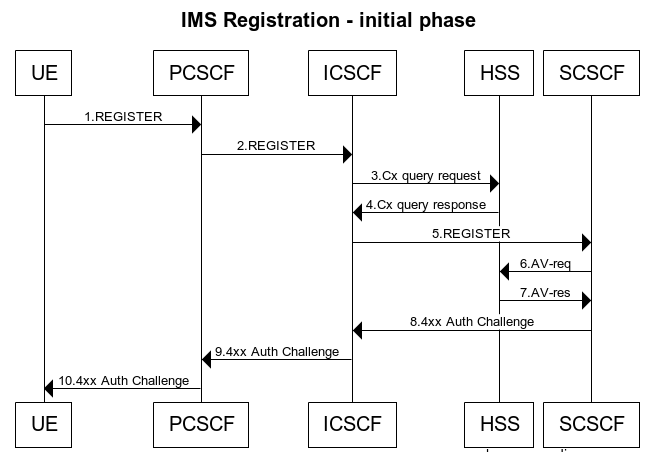
\includegraphics[scale=0.5]{IMS_Registration_0.png} 
\caption{Registration request - initial phase }
\label{fig2}

\end{center}
\end{figure}
In the figure \ref{fig2} we can see sequence diagram of the initial phase of the registration request. 
\begin{enumerate}
\item In REGISTER request, UE sends registration information flow - containing IMSI, UE IP address, an instance identifier, home network name to P-CSCF. 
\item Based on which network this UE belongs to by looking up home network name, P-CSCF will connect to I-CSCF and forwards REGISTER request to ICSCF. P-CSCF will mark the packet as not integrity protected. This integrity protected flag is used by I-CSCF and S-CSCF to check which phase of registration is going on. 
\item I-CSCF will send cx query to HSS, asking for which S-CSCF it should contact. HSS will look up in its database to find out which S-CSCF is assigned to this user. 
\item HSS will look up IMSI and send S-CSCF address to I-CSCF where I-CSCF should send registration request. If it is necessary to select new S-CSCF, it will return required capabilities to I-CSCF.
\item If capabilities are returned, I-CSCF shall construct a name from capabilities returned. Now using S-CSCF name, I-CSCF will get an address of S-CSCF and forward REGISTER message to S-CSCF.
\item S-CSCF will send AV-req (Authentication vector request) message to HSS. 
\item HSS will respond with parameters which are required for authentication in AV-response message.
\item S-CSCF will send back 4xx authentication challenge message to I-CSCF, signifying that UE needs to be authenticated and store relevant parameters.
\item I-CSCF will forward 4xx authentication challenge to P-CSCF. I-CSCF will store relevant parameters. 
\item P-CSCF will store relevant parameters. It will remove parameters which need not be sent to UE. Then it will forward 4xx authentication challenge message to UE.
\end{enumerate}
\subsubsection{Registration request - phase 2}
\begin{figure}[!htbp]
\begin{center}
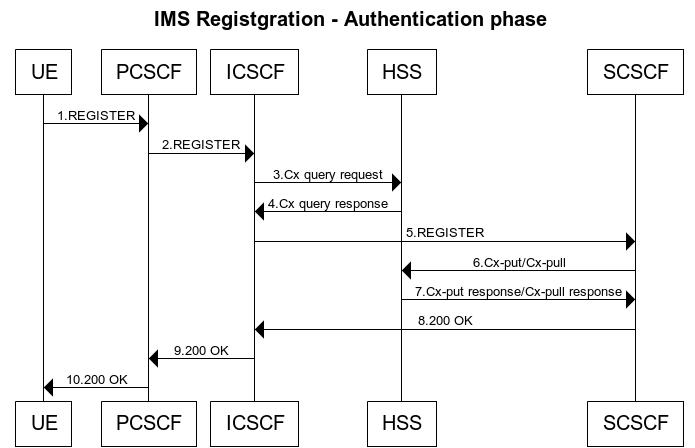
\includegraphics[scale=0.5]{IMS_Registration_2.png} 
\caption{Registration request - authentication phase}
\label{fig3}
\end{center}
\end{figure}
In the figure \ref{fig3} we can see sequence diagram of authentication phase of the registration request. 
\begin{enumerate}
\item Before sending the request, UE will calculate authentication response - RES. In REGISTER request, UE sends registration information flow - containing IMSI, UE IP address, an instance identifier, home network name to P-CSCF along with RES.
\item Based on which network this UE belongs to, by looking up home network name, P-CSCF will connect to I-CSCF and forwards REGISTER request to ICSCF. 
\item I-CSCF will send cx query to HSS, asking for which S-CSCF it should contact. HSS will look up in its database to find out which S-CSCF is assigned to this user. 
\item HSS will look up IMSI and returns S-CSCF name where I-CSCF should send registration request. 
\item Using S-CSCF name, I-CSCF will get an address of S-CSCF and forward REGISTER message to S-CSCF.
\item S-CSCF will retrieve XRES stored at the time of sending the 4xx authentication challenge to UE. It will compare RES returned by UE with XRES. If RES=XRES then the user has been authenticated successfully. It will then send Cx put request to update registration flag on HSS to registered, along with GRUU(Globally Routable User Agent URI) which is just created.
\item HSS will update the registration flag and reply success to S-CSCF. It will store GRUU for that IMSI.
\item Now at this point registration request is complete. S-CSCF will send back 200 OK message to I-CSCF. S-CSCF will store GRUU.
\item I-CSCF will forward 200 OK message to P-CSCF. I-CSCF will release all registration information at this point.
\item P-CSCF will store GRUU. It will forward 200 OK message to  UE.
\end{enumerate}


\subsection*{De-registration}
\begin{figure}[!htbp]
\begin{center}
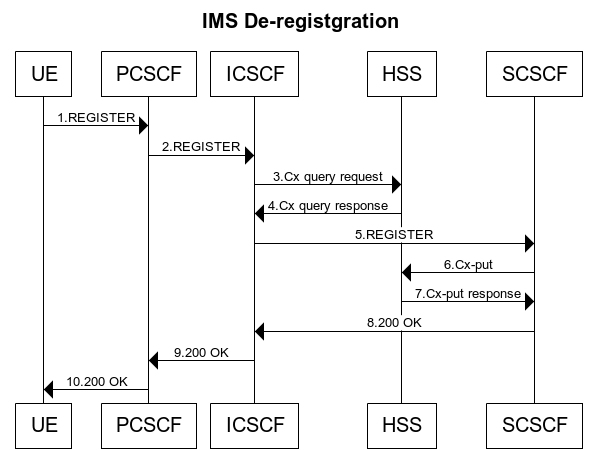
\includegraphics[scale=0.65]{IMS_De-Registration_1.png} 
\caption{De-registration request }
\label{fig4}
\end{center}
\end{figure}
In the Figure \ref{fig4} we can see sequence diagram of deregistration request. 
\begin{enumerate}
\item Deregistration is accomplished by registration with expiration value of 0 seconds. In REGISTER request, UE sends registration information flow - containing IMSI, UE IP address, an instance identifier, home network name to P-CSCF.
\item Based on which network this UE belongs to by looking up home network name, P-CSCF will connect to I-CSCF and forwards REGISTER request to I-CSCF. 
\item I-CSCF will send Cx query to HSS, asking for which S-CSCF it should contact. HSS will look up in its database to find out which S-CSCF is assigned to this user. 
\item HSS will look up IMSI and return S-CSCF name where I-CSCF should send deregistration request.
\item I-CSCF will get an address of S-CSCF and forward REGISTER message to S-CSCF.
\item S-CSCF will send the Cx-put request to HSS. 
\item HSS will clear S-CSCF name for that IMSI and send the Cx-put response to S-CSCF.
\item S-CSCF will send back 200 OK message to I-CSCF. S-CSCF releases all registration information related to this UE.
\item I-CSCF will forward 200 OK message P-CSCF. 
\item P-CSCF will forward 200 OK message to UE. P-CSCF releases all registration information related to this UE.
\end{enumerate}

\section*{Source code overview}
In this part, we describe each of the source code files ( .cpp / .h ), and the various functions involved in it.
PCSCF, ICSCF, SCSCF, HSS use epoll based architecture which was described previously.

\subsection*{PCSCF}
P-CSCF is the first endpoint where all UE requests are initially sent. Based upon the home
network address of UE, P-CSCF determines I-CSCF where the request will be forwarded.
P-CSCF is responsible for forwarding request to I-CSCF of the home network of UE.

\subsection*{ICSCF}
For every registration request, I-CSCF sends a query to HSS, asking for the name of S-CSCF
where UE’s request should be forwarded. I-CSCF will retrieve S-CSCF address and forward
request towards S-CSCF. 

\subsection*{SCSCF}
S-CSCF retrieves authentication vector from HSS after getting the request from I-CSCF and
stores XRES. It sends the authentication challenge to UE. When it received the authentica-
tion response from UE (via I-CSCF), it compares XRES = RES to complete authentication
procedure. If authentication procedure is complete, it updates the status of UE to registered
in HSS. After getting de-registration request, S-CSCF will send the request to HSS to change
the status of UE to unregistered. Then it will remove all registration information and send
200 OK to I-CSCF.

\subsection*{HSS}
HSS which stores IMSI, authentication and random token
information of UE in memory. It also stores registration status information in memory.

\subsection*{common.h}
It contains IP addresses and port numbers of all components of IMS core. And other parameters like maximum events generated. 

\subsection*{SIP}
Used for creating a dummy header for SIP protocol. It is used for identifying which type of request is currently being processed. 

\paragraph*{NOTE:}  Code for following components was adapted from NFV LTE EPC. \\
Link: https://github.com/networkedsystemsIITB/NFV\_LTE\_EPC

\subsection*{NETWORK}
Contains frequently used functions for socket programming. The implemented functions receive various input param-
eters along with a socket file descriptor and perform related functions on the received socket file descriptor. 

\subsection*{PACKET}
A template for generating packets. Each PACKET object denotes a packet, where len denotes the size of the data in
the packet and data ptr denotes the last index position of the packet. The parameter data ptr will be helpful
while adding/reading/removing the packet data. It contains various functions to modify the packet contents.

\subsection*{RAN}
RAN module stores RAN contexts of various objects. It implements functions for registration,authentication and deregistration.

\subsection*{RAN SIMULATOR}
Main function for the RAN module. It creates multiple RAN objects for generating control traffic and  responsible for computing various performance metrics for traffic experimentation.

\subsection*{SCTP CLIENT}
A simple stream oriented client program that has functions for connecting to a server, sending and receiving SCTP packets

\subsection*{SECURITY}
Contains classes for encryption and integrity check. Both uses the built-in functions of openssl that perform encryption,
decryption and HMAC digest generation. AES 256 CBC algorithm is used for encryption/decryption and EVP SHA1
algorithm is used for integrity check. Sample key and iv values are used for all algorithms; Implemented functions
are straightforward to understand.

\subsection*{TELECOM}
Contains functions for computing various telecom parameters such as IMSI and GRUU. Standard
pattern is used for computing all parameters.

\subsection*{UTILS}
A common program employed by all the modules. Contains most frequently used functions such as error checking
and allocating memory.

\subsection*{SYNC}
Contains pthread functions for initializing mutex, locking/unlocking mutex and wait/signal on mutex. Imple-
mented functions are straightforward to understand.	

\end{document}
